%%
% This is an Overleaf template for presentations
% using the TUM Corporate Desing https://www.tum.de/cd
%
% For further details on how to use the template, take a look at our
% GitLab repository and browse through our test documents
% https://gitlab.lrz.de/latex4ei/tum-templates.
%
% The tumbeamer class is based on the beamer class.
% If you need further customization please consult the beamer class guide
% https://ctan.org/pkg/beamer.
% Additional class options are passed down to the base class.
%
% If you encounter any bugs or undesired behaviour, please raise an issue
% in our GitLab repository
% https://gitlab.lrz.de/latex4ei/tum-templates/issues
% and provide a description and minimal working example of your problem.
%%


\documentclass[
  english,            % define the document language (english, german)
  aspectratio=169,    % define the aspect ratio (169, 43)
  % handout=2on1,       % create handout with multiple slides (2on1, 4on1)
  % partpage=false,     % insert page at beginning of parts (true, false)
  % sectionpage=true,   % insert page at beginning of sections (true, false)
]{tumbeamer}


% load additional packages
\usepackage{booktabs}
\usepackage{graphicx}
\usepackage{subcaption}
\usepackage{amsmath, amsthm}

% presentation metadata
\title{Seminar: Convex Geometry}
\subtitle{Approximation of Convex Bodies and Applications}
\author{Ao Wei}

\institute{\theDepartmentName\\\theUniversityName}
\date[12/06/2025]{June 12\textsuperscript{th}, 2025}

\footline{\insertauthor~|~\insertshorttitle~|~\insertshortdate}


% macro to configure the style of the presentation
\TUMbeamersetup{
  title page = TUM tower,         % style of the title page
  part page = TUM toc,            % style of part pages
  section page = TUM toc,         % style of section pages
  content page = TUM more space,  % style of normal content pages
  tower scale = 1.0,              % scaling factor of TUM tower (if used)
  headline = TUM threeliner,      % which variation of headline to use
  footline = TUM default,         % which variation of footline to use
  % configure on which pages headlines and footlines should be printed
  headline on = {title page},
  footline on = {every page, title page=false},
}

% available frame styles for title page, part page, and section page:
% TUM default, TUM tower, TUM centered,
% TUM blue default, TUM blue tower, TUM blue centered,
% TUM shaded default, TUM shaded tower, TUM shaded centered,
% TUM flags
%
% additional frame styles for part page and section page:
% TUM toc
%
% available frame styles for content pages:
% TUM default, TUM more space
%
% available headline options:
% TUM empty, TUM oneliner, TUM twoliner, TUM threeliner, TUM logothreeliner
%
% available footline options:
% TUM empty, TUM default, TUM infoline

% theorem mark numbers
\newtheorem{theorem}{Theorem}
\newtheorem{lemma}{Lemma}
\newtheorem{corollary}{Corollary}

\begin{document}

\maketitle

\section{Löwner-John's Ellipsoids}

\begin{frame}{Introduction to John's Ellipsoids}{John's Theorem}
    \begin{center}
    \begin{theorem}[John's Ellipsoid Theorem]
      Let $C \subset\mathbb{R}^d$ be a convex body. Then there exists an ellipsoid $E$ (called the \textbf{John ellipsoid}) such that if $c$ is the center of $E$, then the following inclusions hold:
    \[
    E \subseteq C \subseteq c + d(E - c),
    \]
    In particular, if $C$ is symmetric in origin, then the tighter bound holds:
    \[
    E \subseteq C \subseteq c + \sqrt{d}(E - c),
    \]
    \end{theorem}
  \end{center}
\end{frame}

\begin{frame}{Introduction to John's Ellipsoids}{2d samples}
  \begin{itemize}
    \item Asymmetric
  \end{itemize}
  \begin{figure}
      \centering
      \begin{subfigure}[b]{0.4\textwidth}
        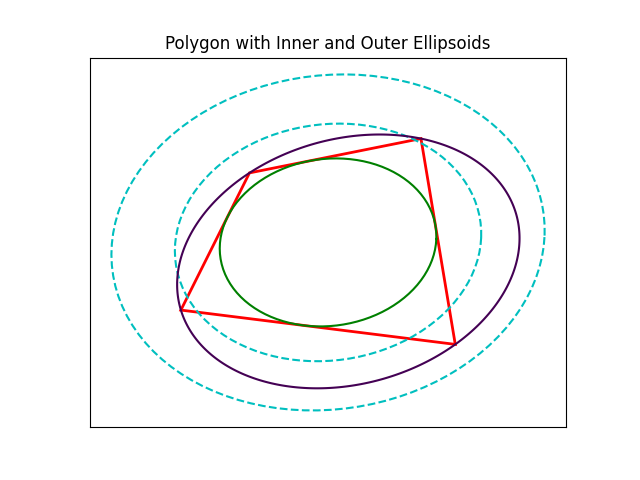
\includegraphics[width=\textwidth]{plots/asym_1.png}
      \end{subfigure}
      \begin{subfigure}[b]{0.4\textwidth}
        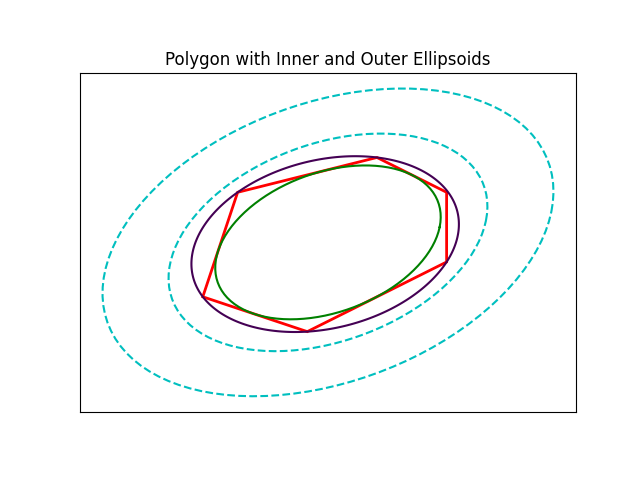
\includegraphics[width=\textwidth]{plots/asym_2.png}
      \end{subfigure}
       \label{fig:enter-label}
  \end{figure}
\end{frame}

\begin{frame}{Introduction to John's Ellipsoids}{2d samples}
  \begin{itemize}
    \item Symmetric
  \end{itemize}
  \begin{figure}
    \centering
    \begin{subfigure}[b]{0.4\textwidth}
        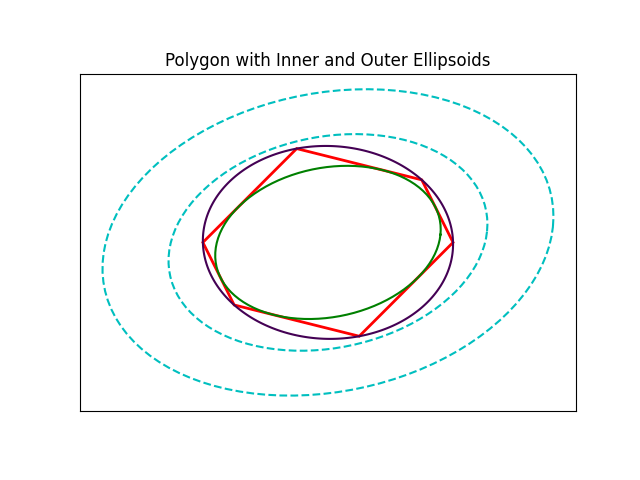
\includegraphics[width=\textwidth]{plots/sym_1.png}
    \end{subfigure}
    \begin{subfigure}[b]{0.4\textwidth}
        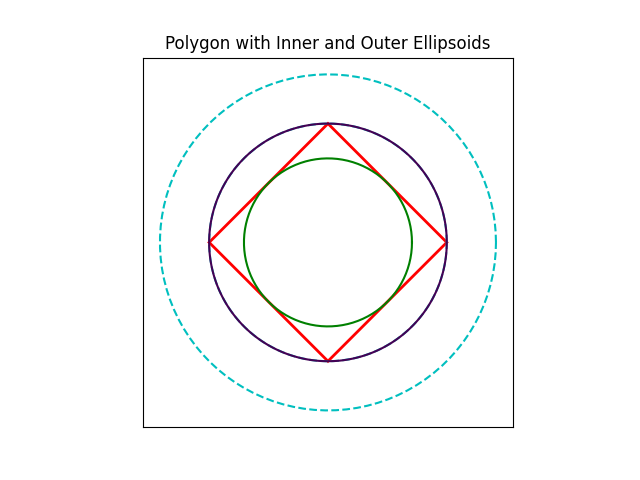
\includegraphics[width=\textwidth]{plots/sym_2.png}
    \end{subfigure}
  \end{figure}
\end{frame}

\begin{frame}{Uniqueness and John's Characterization Theorem}
\centering
\begin{theorem}
  If $C \subset R^{d}$ be a convex body, then the inner ellipsoid of maximal volume is unique.
\end{theorem}
\begin{theorem}[]

\end{theorem}
\end{frame}

\begin{frame}{John's Characterization Theorem}{$B^{d}$ as inner John's Ellipsoid}

\end{frame}

\begin{frame}{Proof Sketch}

\end{frame}

\begin{frame}{Group of Affinities of a convex body}

\end{frame}

\begin{frame}{The Banach-Mazur distance}

\end{frame}

\section{Reverse Isoperimetric Inequality}
\begin{frame}{Reverse Isoperimetric Inequality}{Introduction}
  \begin{itemize}
    \item Recall: Isoperimetric Inequality and its revealed fact
    \item What does reverse isoperimetric Inequality show?
    \item Isoperimetric quotient
  \end{itemize}
\end{frame}

\begin{frame}{Reverse Isoperimetric Inequality}{Ball vs. Cube by n-dims}

\end{frame}

\begin{frame}{Proof of Reverse Isoperimetric Inequality}{using John's Characterization Theorem}
Brascamp–Lieb inequality:

\end{frame}

\section{Asymptotic best Approximation by Polytopes}
\begin{frame}{Polytope Approximation of Ellipsoid}{2d example}
  \begin{itemize}
    \item Recall:Best approximated n-polygon in Circle is Regular Polygon 
    \item ellipse is circle after affine transformation.
    \item Easy to see here: Best approximated n-polygon in Ellipse is Regular n-polygon after the affine transformation
  \end{itemize}
\end{frame}

\begin{frame}{Polytope Approximation of Ellipsoid}{other dimensions: hard!}
 Though Ellipsoid is still an affine transformation of Ball, It's already hard to find the best n-facets polytope in $B^{d}$
 \\
 See the reference:
  \begin{itemize}
     \item https://math.stackexchange.com/questions/979660/largest-n-vertex-polyhedron-that-fits-into-a-unit-sphere
     \item https://arxiv.org/abs/1402.6496
  \end{itemize}
\end{frame}


\begin{frame}{Asymptotic Formula}{Introduction}
    \begin{itemize}
        \item Estimate the difference:$\delta(C,Q_{n})$
        \item Symmetric difference: $\delta^{V}(C,D)$
    \end{itemize}
\end{frame}

\begin{frame}{Asymptotic Formula}{Proof Ideas}
    \begin{itemize}
        \item Prove the lower bound: Use local quadratic approximation, apply Zador's theorem, and do global integration
        \item Prove the upper bound: To construct a specific polytope achieving this rate by doing curvature-weighted sampling, build circumscribed polytope and estimate volume excess
    \end{itemize}
\end{frame}

\begin{frame}{Isoperimetric Problem for Convex Polytopes}
  \begin{itemize}
    \item To describe the polytope $P_{n} \in \mathcal{P}_{n}$ with minimum isoperimetric quotient, which is a consequence of the above approximation theorem
  \end{itemize}
\end{frame}


\section{Heurisitic Principle}
\begin{frame}{Approximated by random polytopes}
    
\end{frame}
\begin{frame}{Heurisitic Observations}
  \begin{itemize}
    \item In many complicated situations, for example in high dimensions or depending on many parameters, average configurations are almost extremal or attain almost the mean value or the median
  \end{itemize}
\end{frame}

\begin{frame}[plain]
  \centering
  \vfill
  {\Huge \textbf{Thanks and Q\&A}}
  \vfill
\end{frame}

\end{document}
